\documentclass[12pt, a4paper]{article}
\usepackage{graphicx}
\graphicspath{ {./imgs/} }
\usepackage{float}
\usepackage{listings}
\usepackage{color}

\definecolor{codegreen}{rgb}{0,0.6,0}
\definecolor{codegray}{rgb}{0.5,0.5,0.5}
\definecolor{codeorange}{rgb}{1,0.49,0}
\definecolor{backcolour}{rgb}{0.95,0.95,0.96}

\lstset{
  backgroundcolor=\color{backcolour},   
  commentstyle=\color{codegray},
  keywordstyle=\color{codeorange},
  numberstyle=\tiny\color{codegray},
  stringstyle=\color{codegreen},
  basicstyle=\ttfamily\footnotesize,
  breakatwhitespace=false,         
  breaklines=true,                 
  captionpos=b,                    
  keepspaces=true,                 
  numbers=left,                    
  numbersep=5pt,                  
  showspaces=false,                
  showstringspaces=false,
  showtabs=false,                  
  tabsize=2,
  xleftmargin=10pt,
}
\renewcommand{\lstlistingname}{Code}

\counterwithin{figure}{section}

%to write code:
%\begin{lstlisting}[language=java, caption={my caption}]
%    
%\end{lstlisting}

%to insert an image
%\begin{figure}[H]
%  \centering
%  \includegraphics[width=\columnwidth]{img.png}
%  \caption{description of the image}
%\end{figure}

\title{Web Architectures - Delivery 5}
\author{Marrocco Simone}

\begin{document}
  \maketitle
  \begin{figure}[H]
    \centering
    
\includegraphics[scale=0.35]{unitn.png}
  \end{figure}
  \tableofcontents
  \pagebreak

  \section{The assignment}
  Our task was to create a Front End application that works with the Scottish Parlament API using Angular. There are two pages: the first one shows all the members. When clicking a particular member, a new page opens showing more data about her/him.

  \section{Tecnology used}
  The project was created with the \textbf{ng} command line interface, using the \textbf{ng new} command. To start the application it was used \textbf{ng serve}, to create a new component \textbf{ng generate component X}, and to build the files to use in production \textbf{ng build}.

  To write the code it was used VScode because of its compatibility with typescript and the aviable addons. The code is also loaded on a repo, visitable at \\
  \textbf{https://github.com/Marrocco-Simone/AngularScottishParlamentFE}

  Github allows the users to serve the content from a repository to a static website, so the best way to look up at the project is by going to \\
  \textbf{https://marrocco-simone.github.io/AngularScottishParlamentFE/}
  
  There were some problem with the Angular build, used later with the Tomcat server: in the \textbf{index.html} it is generate a tag \textbf{\textless base href="/"\textgreater} which does not allow the web browser to find the javascript files if not hosted on a basic url (like \textbf{localhost:4200/}) but instead on a sub page (like \textbf{localhost:4200/AngularWarExploded/}). The solution is change the tag to \textbf{\textless base href="."\textgreater}, but this means it is not possible to just use the builded files directly. For more information, you can look at \\
  \textbf{https://stackoverflow.com/questions/50858981/html-relative-paths-issue-for-script-src}

  \pagebreak
  \section{The final website}

  The CSS is aviable in the source code

  \begin{figure}[H]
    \centering
    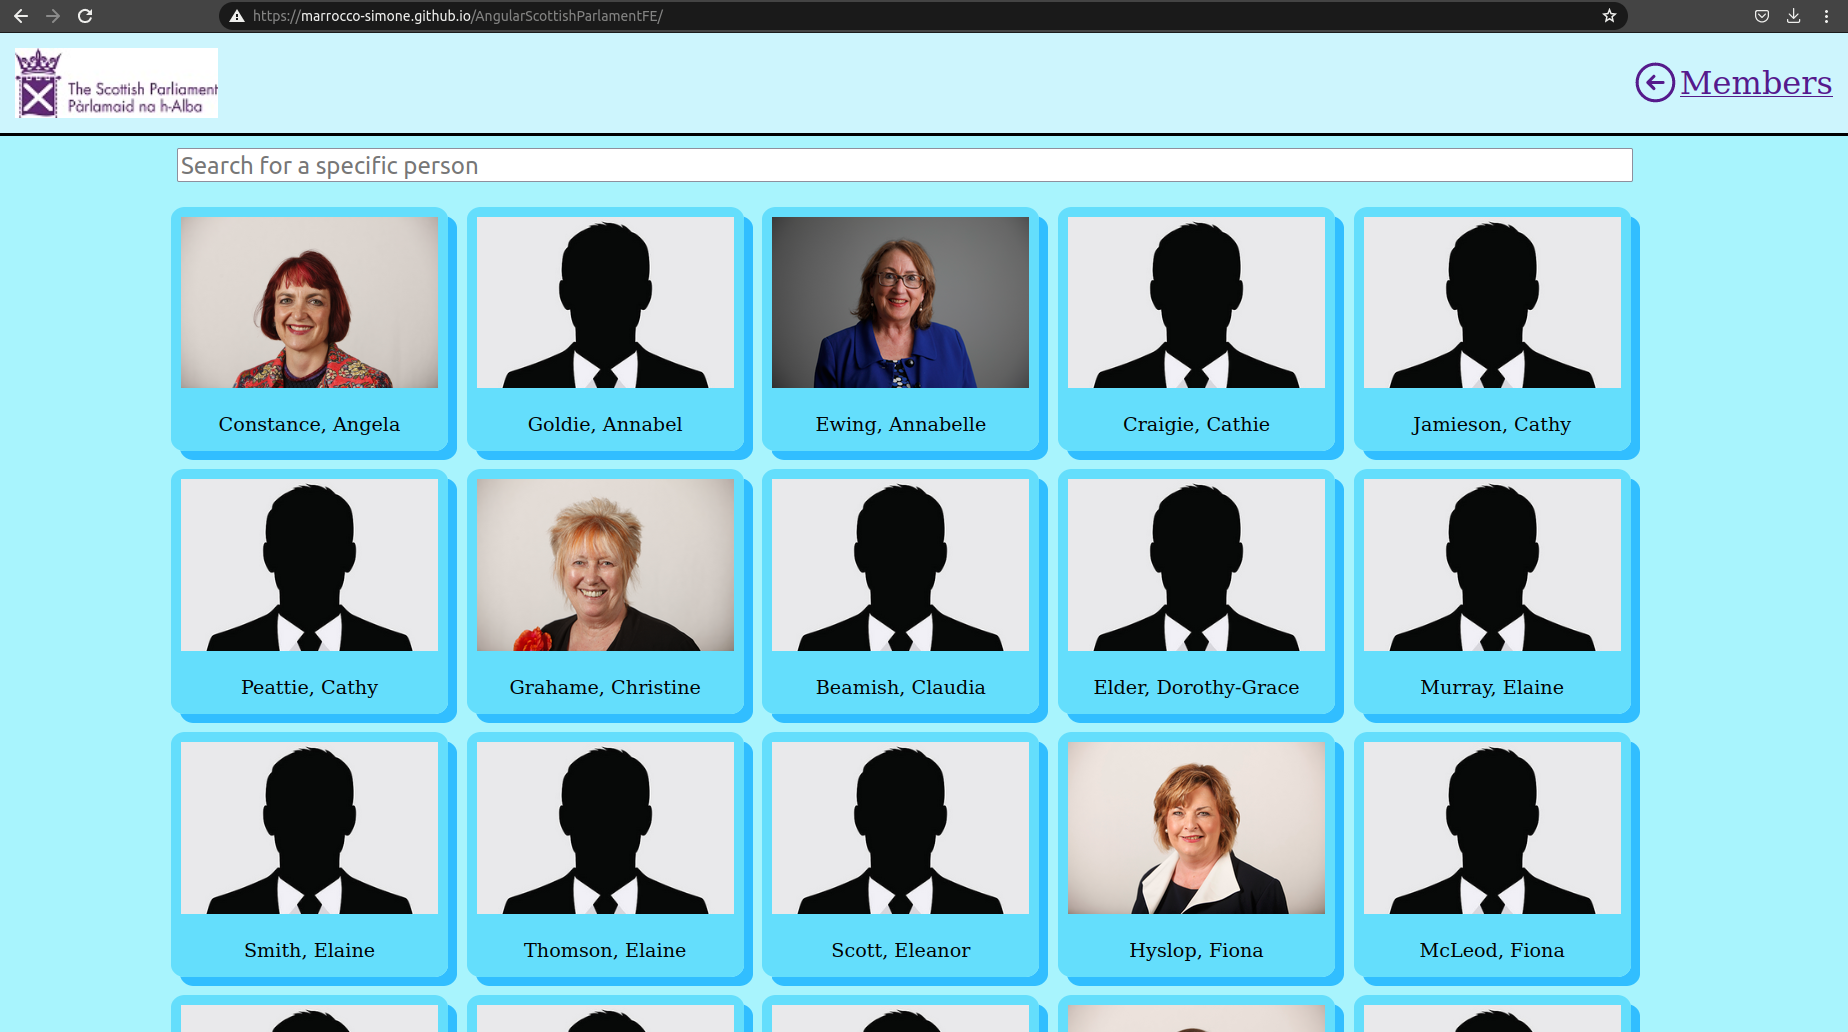
\includegraphics[width=\columnwidth]{main.png}
    \caption{Main Page}
  \end{figure}
  \begin{figure}[H]
    \centering
    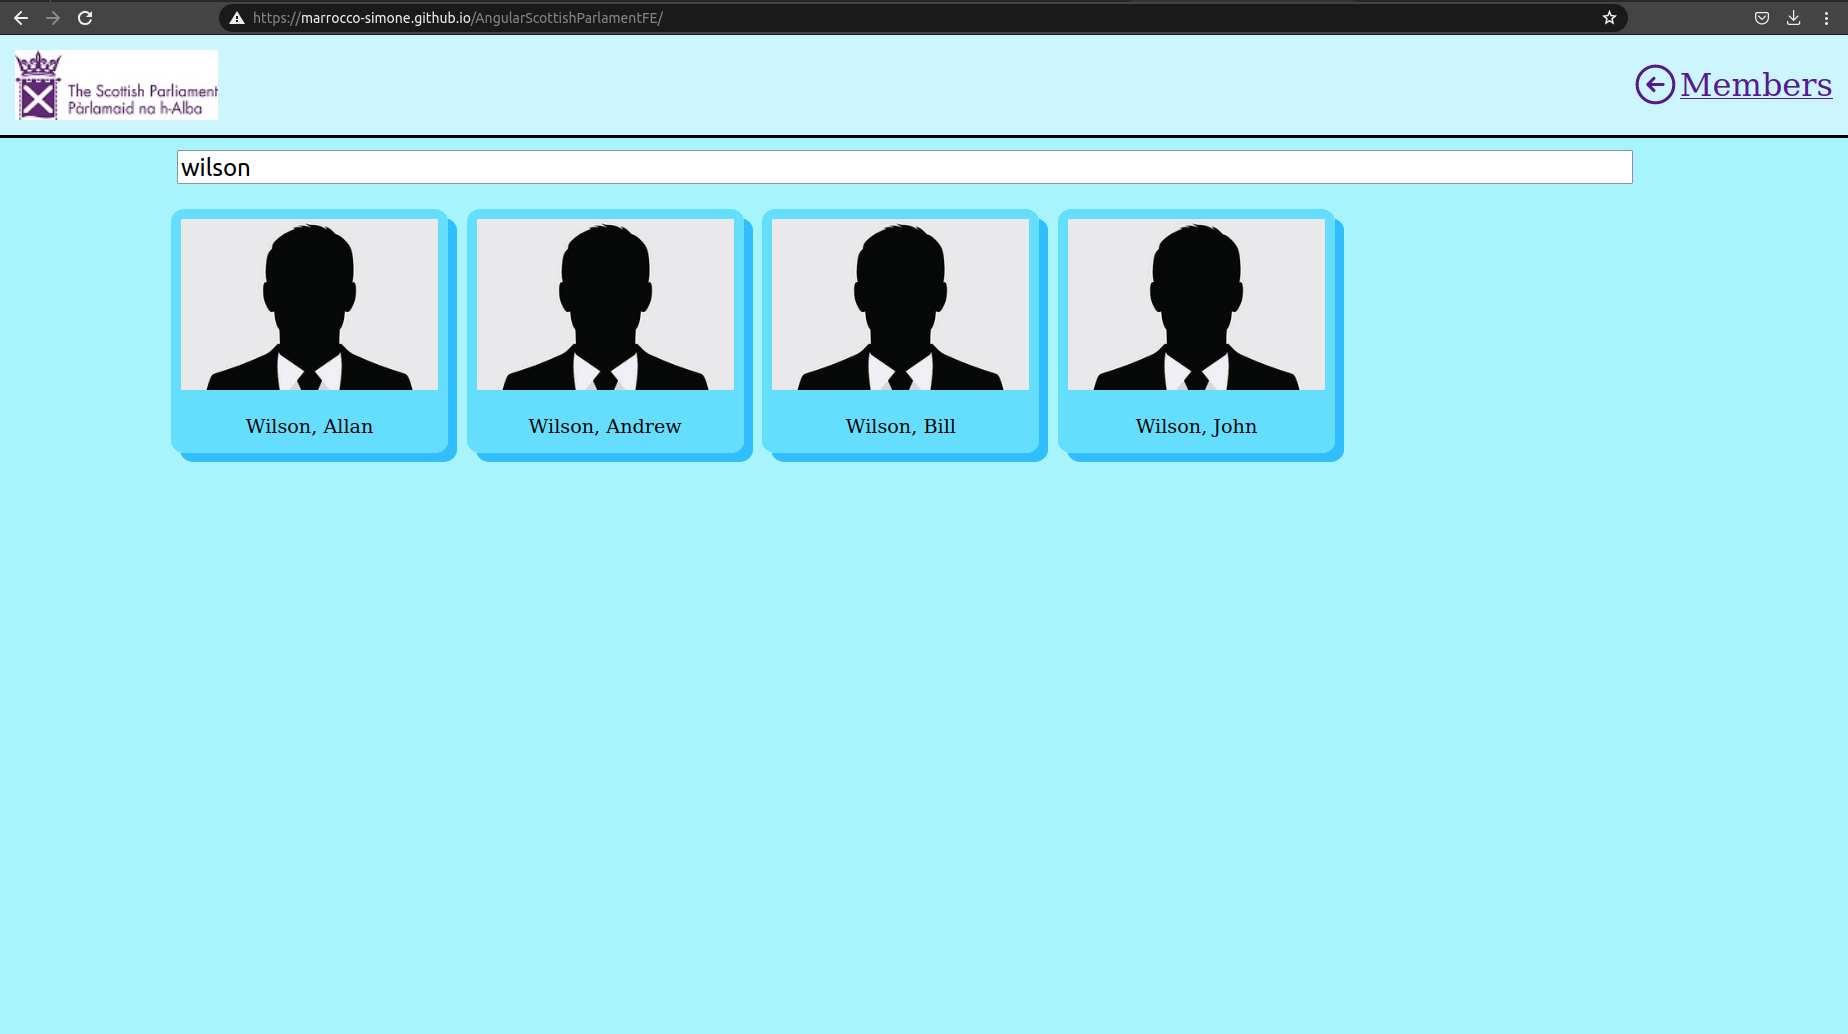
\includegraphics[width=\columnwidth]{search_bar.png}
    \caption{Searching for a member}
  \end{figure}
  \begin{figure}[H]
    \centering
    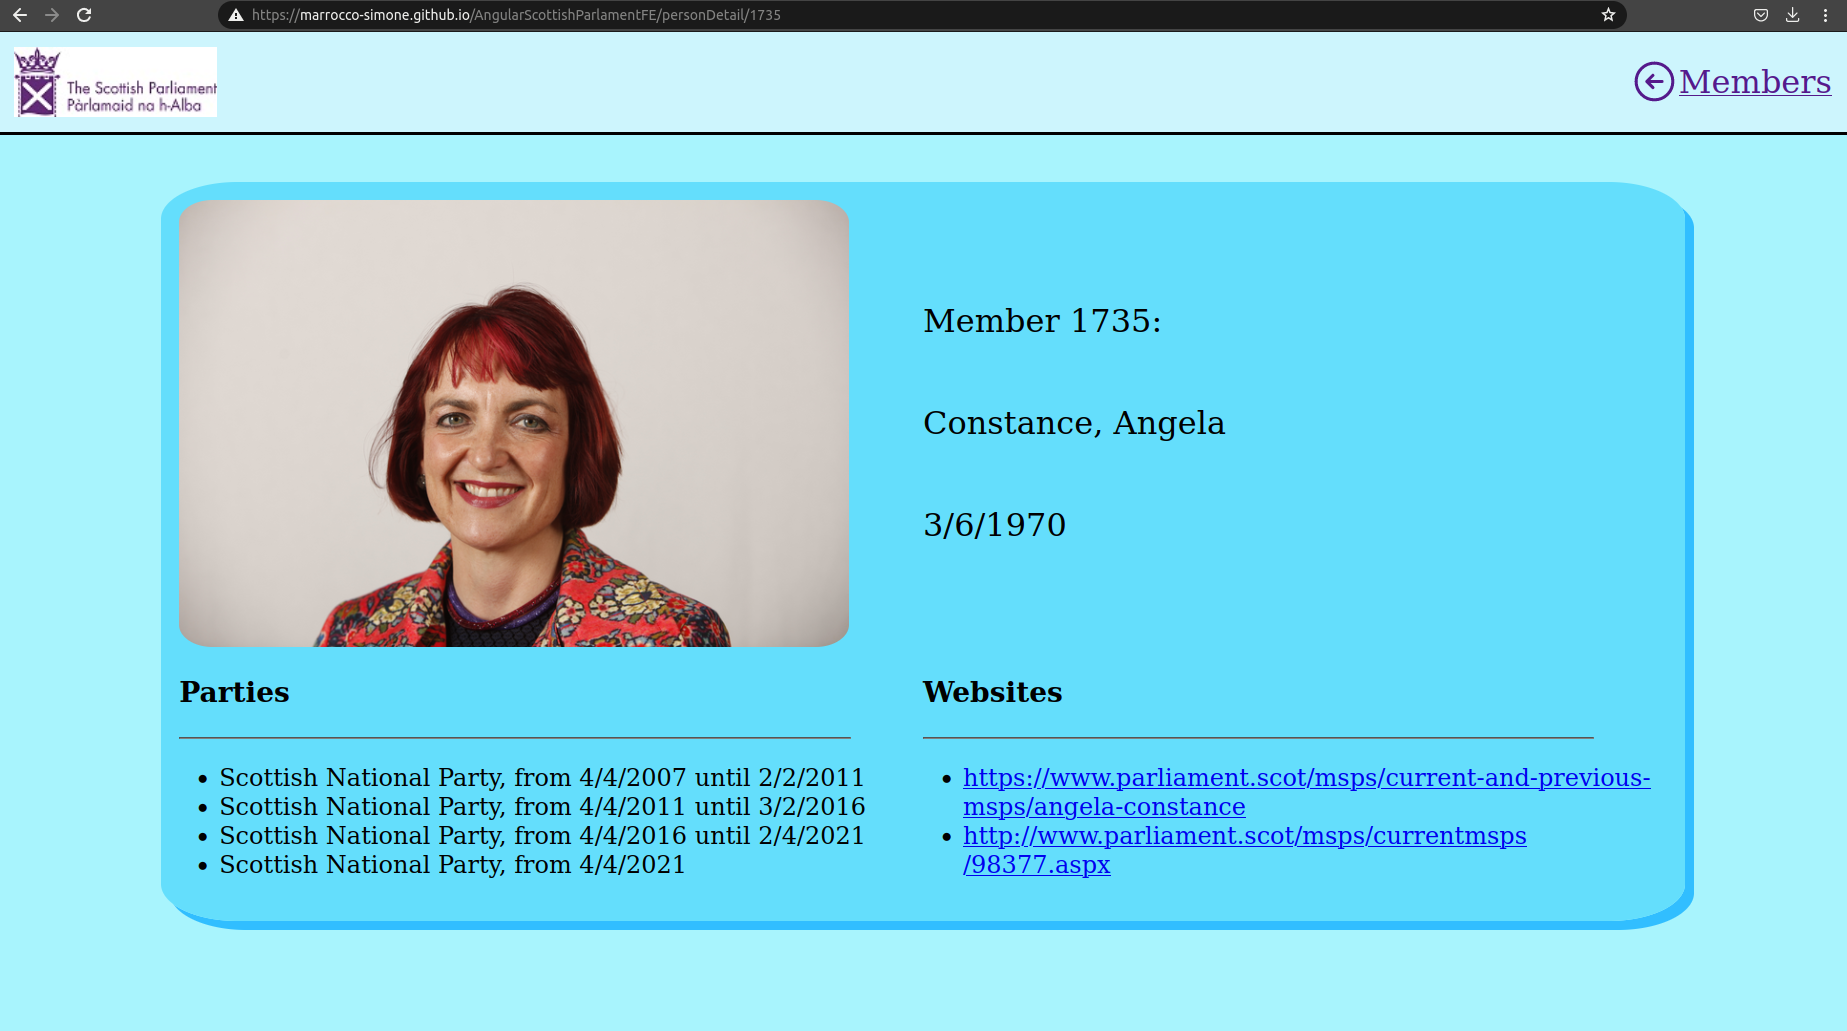
\includegraphics[width=\columnwidth]{full.png}
    \caption{Person Detail Page}
  \end{figure}

  \pagebreak
  \section{App component}
  \begin{lstlisting}[language=html, caption={App component html}]
    <app-header></app-header>
    <router-outlet></router-outlet>\end{lstlisting}

  The HTML of the top component is quite simple: we load an header on top and we inject the router, which will choose what component to load.

  \subsection{Header component}

  \begin{lstlisting}[language=html, caption={Header component constructor}]
    <header>
      <img src="https://data.parliament.scot/Content/Images/SP_145_50.jpg" />
      <a routerLink="/">
        <svg></svg>    
        Members
      </a>
    </header>\end{lstlisting}
  
  In the header, we load the scottish parlament logo taken from their website and an hyperlink redirecting to the first page, enriched with an svg (not shown here). The redirect is done with the router.

  \subsection{Router}
  \begin{lstlisting}[language=java, caption={Router component module}]
    const routes: Routes = [
      { path: "", component: MainComponent },
      { path: "personDetail/:personId", component: FullPersonComponent}
    ];

    @NgModule({
      imports: [RouterModule.forRoot(routes)],
      exports: [RouterModule]
    })
    export class AppRoutingModule { }\end{lstlisting}

  In the router we define two pages: the main page, located on /, uses the main component. The second page, showing the full person details, uses a dynamic link with the person ID to load the requested member (we will see later how to recover in the component this id from the url).

  \pagebreak
  \section{API data and services}

  We have three services, used to get the members, their parties and their websites. Each service has a constructor, which calls async functions to fetch the data from the API server, and some functions that work with the data they hold.

  The member service is called on the main component constructor. The rest of the data, about the people websites and parties, is loaded only when it is needed, as the client clicks on one of the members to go to the detail page. It is possible to verify when the data is fetch by pressing f12, since console logs are added to show that it works as intended (if you're looking on the github page, remember to turn off the warning messages)
  
  Unfortunately, there is no API to get only a single person data, so we need to get the full list for everyone. However, this means that after the first click the rest of them are going to load instantly.

  \begin{lstlisting}[language=java, caption={Websites API Service}]
    export class WebsitesService {
      private websites!: Website[];

      private async getWebsites() {
        console.log('fetching websites');
        let res = await fetch(websitesApiUrl);
        this.websites = await res.json();
      }

      constructor() {
        this.getWebsites();
      }

      getWebsiteUrls(personId: string): string[] {
        if (!this.websites?.length) return [];
        return this.websites
          .filter((w) => `${w.PersonID}` == personId)
          .map((w) => w.WebURL);
      }
    }\end{lstlisting}

  \pagebreak
  \begin{lstlisting}[language=java, caption={Members API Service}]
    export class MembersService {
      members: Member[] = [];

      private async getMembers() {
        console.log('fetching members');
        let res = await fetch(membersApiUrl);
        this.members = await res.json();
      }

      constructor() {
        this.getMembers();
      }

      getSingleMember(personId: string) {
        return this.members.find((m) => `${m.PersonID}` == personId);
      }

      getProfilePicture(member: Member) {
        let url = member.PhotoURL
          ? member.PhotoURL
          : 'assets/blank-profile-picture.jpg';
        return url;
      }

      getBirthDate(member: Member) {
        if (!member.BirthDate) return '';
        try {
          let date = new Date(member.BirthDate);
          return `${date.getDay()}/${date.getMonth()}/${date.getFullYear()}`;
        } catch (e) {
          return '';
        }
      }
    }\end{lstlisting}
  
  \begin{lstlisting}[language=java, caption={Parties API Service}]
    export class PartiesService {
    private parties!: Party[];
    private members_parties!: MemberParties[];

    private async getParties() {
      console.log('fetching parties');
      let res = await fetch(partiesApiUrl);
      this.parties = await res.json();
    }
 
    
    private async getMembersParties() {
      console.log('fetching member parties');
      let res = await fetch(membersPartyApiUrl);
      this.members_parties = await res.json();
    }

    constructor() {
      this.getParties();
      this.getMembersParties();
    }

    private getPartyName(party_id: number): string {
      if (!this.parties?.length) return "";
      return this.parties.find((mp) => mp.ID == party_id)?.ActualName ?? "";
    }

    getPersonParties(personId: string): string[] {
      if (!this.parties?.length || !this.members_parties?.length) return [];
      let member_parties = this.members_parties.filter((mp) => `${mp.PersonID}` == personId);
      let parties_names: string[] = [];
      
      for (let pmp of member_parties) {
        let party_name = this.getPartyName(pmp.PartyID);
        if (!party_name) continue;

        if (pmp.ValidFromDate) {
          let date = new Date(pmp.ValidFromDate);
          party_name += `, from ${date.getDay()}/${date.getMonth()}/${date.getFullYear()}`;
        }
        if (pmp.ValidUntilDate) {
          let date = new Date(pmp.ValidUntilDate);
          party_name += ` until ${date.getDay()}/${date.getMonth()}/${date.getFullYear()}`;
        }

        parties_names.push(party_name);
      }

      return parties_names;
    }
  }\end{lstlisting}

  \pagebreak
  \section{Main component}

  In the main component, we make full use of the power of angular in creating dynamic pages with very little code.

  The page has two main parts: the search bar and the grid of members.

  The search bar is made of an input tag where we intercept the key-pressed event and save the text value in a variable.

  For the grid of members, we cycle through each one and show it if the member name contains the searched value. Of course, if the bar is empty all the members will be shown, since every string contains the null one. The way of showing a single member is leaved to another component, to which we pass the member data.

  \begin{lstlisting}[language=java, caption={Main component}]
    export class MainComponent {
      inputSearchValue = '';

      constructor(public membersService: MembersService) {}

      onKeyPressed(event: any) {
        this.inputSearchValue = event.target.value;
      }
    }\end{lstlisting}

  \begin{lstlisting}[language=html, caption={Main html}]
    <div class="minimized-people">
      <input
        (keyup)="onKeyPressed($event)"
        placeholder="Search for a specific person"
      />
      <div *ngFor="let m of membersService.members">
        <app-minimized-person
          *ngIf="
            m.ParliamentaryName.toLocaleLowerCase().includes(
              inputSearchValue.toLocaleLowerCase()
            )
          "
          [member]="m"
        ></app-minimized-person>
      </div>
    </div>\end{lstlisting}

  \pagebreak
  \section{Minimized Person component}

  With the member we get as an input from the parent component, this one creates an html link to its detail page, showing the profile picture and the name of the person. The URL for the picture is given from the member service, which returns the blank profile picture image if there is no personal picture.

  \begin{lstlisting}[language=java, caption={Minimized Person component}]
    export class MinimizedPersonComponent {
      @Input()
      member!: Member;

      constructor(public membersService: MembersService) {}
    }\end{lstlisting}

  \begin{lstlisting}[language=html, caption={Minimized Person html}]
    <a [routerLink]="['/personDetail', member.PersonID]" class="minimized-person">
      <img src={{membersService.getProfilePicture(member)}}/>
      <p>{{member.ParliamentaryName}}</p>
    </a>\end{lstlisting}

  \pagebreak
  \section{Full Person component}

  In the full page, we use all the three services (two of which will be initialized when this component is loaded for the first time). In the constructor we get the member ID from the URL and search for the corresponding member. If there is none, the client gets redirected to the main page.

  \begin{lstlisting}[language=java, caption={Full Person component}]
    export class FullPersonComponent {
      member!: Member;
      personId!: string;

      constructor(
        route: ActivatedRoute,
        router: Router,
        public membersService: MembersService,
        public partiesService: PartiesService,
        public websiteService: WebsitesService
      ) {
        route.params.subscribe((params: Params) => {
          this.personId = params['personId'];
          let member = membersService.getSingleMember(this.personId);
          if (!member) {
            router.navigate(['/']);
            return;
          }
          this.member = member;
        });
      }
    }\end{lstlisting}

  \pagebreak
  \begin{lstlisting}[language=html, caption={Full Person html}]
    <div class="full-person">
      <img src="{{ membersService.getProfilePicture(member) }}" />
      
      <div class="full-person-description">
        <p>Member {{ member.PersonID }}:</p>
        <p>{{ member.ParliamentaryName }}</p>
        <p>{{ membersService.getBirthDate(member) }}</p>
      </div>
    
      <div class="full-person-extra-data">
        <h3>Parties</h3>
        <hr>
        <ul>
          <li *ngFor="let party of partiesService.getPersonParties(personId)">{{ party }}</li>
        </ul>
      </div>
      
      <div class="full-person-extra-data">
        <h3>Websites</h3>
        <hr>
        <ul>
          <li *ngFor="let website of websiteService.getWebsiteUrls(personId)">
            <a [href]="website" target="_blank">{{ website }}</a>
          </li>
        </ul>
      </div>
    </div>\end{lstlisting}
\end{document}
